\documentclass[11pt, letterpaper]{article}

\title{Push: a DISC shell}
\author{Noah Evans \\Nara Institute of Science and Technolgoy \\noah-e@is.naist.jp  \and Eric Van Hensbergen \\IBM Research \\bergevan@us.ibm.com}

\usepackage{fullpage}

\usepackage{graphicx}

\date{}

\begin{document}

\maketitle

%maybe lead in with something different
Unix Pipes~\cite{mcilroy1964paf} were a major advance in software engineering, 
allowing the composibility of previously isolated programs regardless of 
programming language. 
With the move to 
Data Intensive Supercomputing (DISC)~\cite{bryant2007dis} 
there is a similar trend towards the use of pipelines in a distributed fashion. 
Runtimes ~\cite{dean2008msd}~\cite{bialecki:hfr}~\cite{isard2007ddd} define 
graphs of processes, the edges of the graphs representing 
pipes and their vertices represent computation on a system.  
With these runtimes and 
a new class of languages~\cite{pike2005idp}~\cite{yu2008dsg}~\cite{olston2008pln} 
built on top of them researchers can solve "pleasantly parallel" 
problems more quickly without worrying about explicit concurrency.

These languages provide automated control flow(typically matched to the 
architecture of the underlying runtime) and channels of communication between 
systems, but none of these languages match the terseness and simplicity of 
the UNIX shell model (e.g. 'sort $|$ uniq -c') which can compose a number of 
smaller programs into a coherent workflow to solve more complicated problems 
quickly. In addition these static workflows are tied to the runtimes that they 
are written on. This makes solutions written for one DISC runtime inherently 
incompatible with other runtimes or languages, tying solutions to a particular 
runtime, workflow and language.

UNIX pipeliens were designed to get around many of these incompatibilities, 
allowing developers to hooks together tools written in different languages and
runtimes.  This allowed tool developers to focus on doing one thing well, and
enabled their code to be portable across versions of the operating system or
architectures.  
Tools read from standard input and wrote to standard output, allowing programs 
to work together in streams \emph{with no explict knowledge of this chaining
built into the program itself}.

We have implemented a shell using Data Intensive SuperComputing(DISC) 
principles, PUSH, which contains built in operators to provision and connect 
virtual and/or physical OS instances.  Process distribution and interconnections 
are composed using synthetic file systems, pushing the distributed complexity 
into the middleware in an language and runtime independent fashion.

\begin{figure}[htp]
\centering
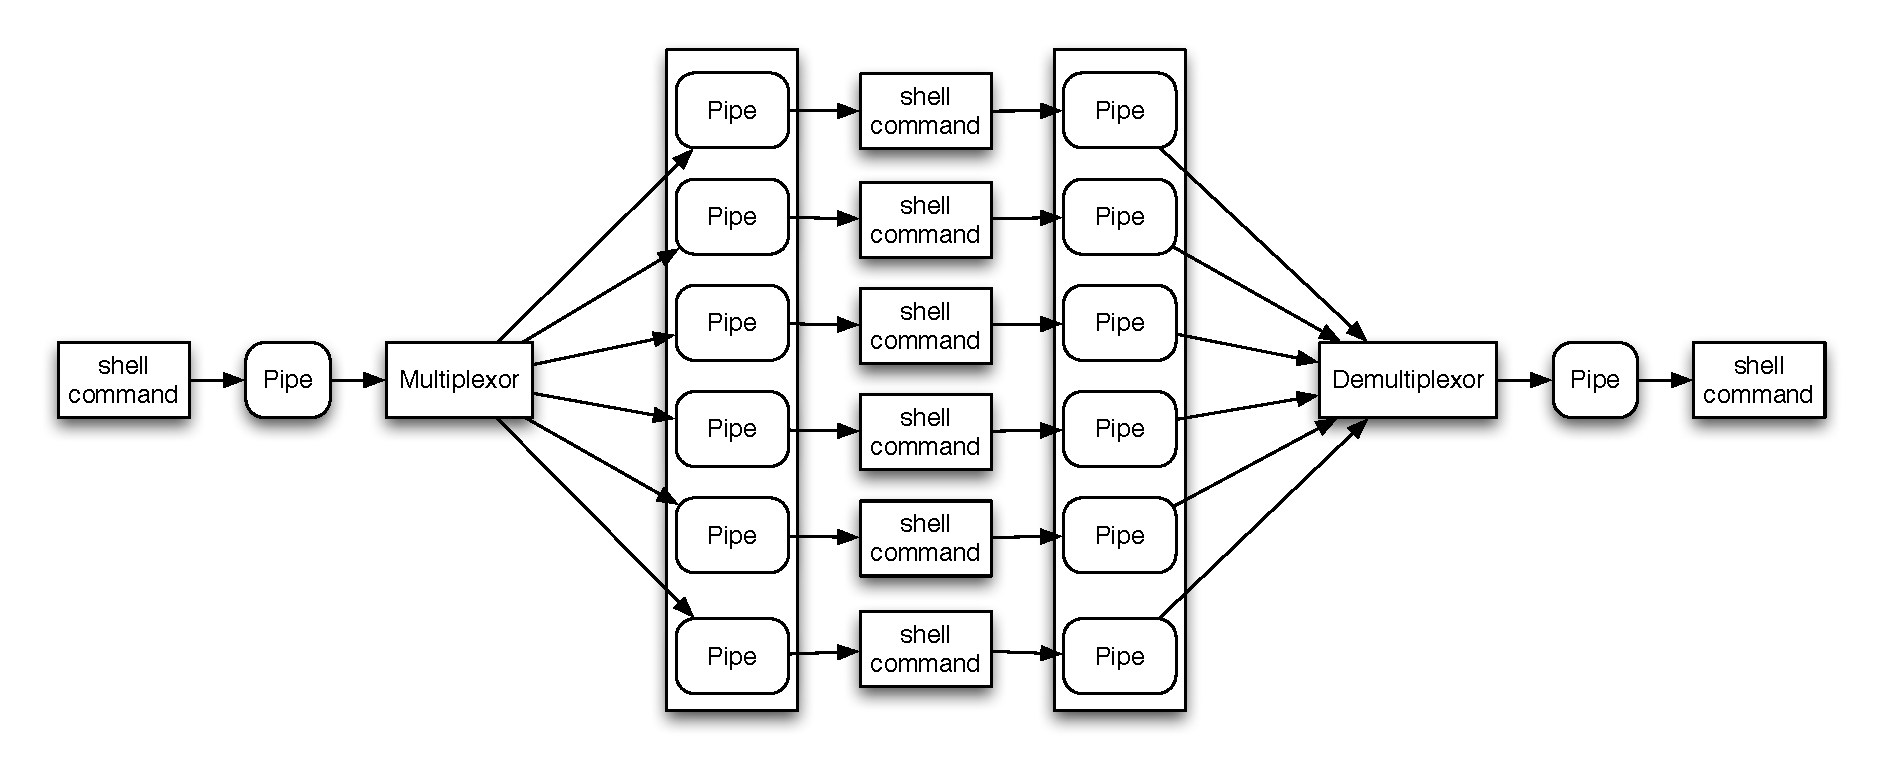
\includegraphics[width=4.5in]{pipestruct.eps}
\caption{The structure of the Push shell. Push implements a new form of multiplexed pipelines which all the distribution of record based output to multiple threads of control. This data is first "Fanned out" to multiple pipes by a multiplexor and then it is subsequently "Fanned in" by a de-multiplexor}\label{fig:pipestruct} 
\end{figure}

However moving to a DISC pattern from the traditional shell model of linear pipelines over bytestreams is nontrivial. 
As \cite{pike2005idp} notes DISC systems need to be able to cleanly separate input streams into records and then show that the order of these records is independent. By separating input and output into discrete unordered records data can be easily distributed and coalesced.

The traditional UNIX way of composing programs is unsuited to this strategy, currently when UNIX programs communicate through pipes they write using buffered byte streams which have no concept of the structure of the underlying data flow. Since UNIX programs write data according to buffer boundaries instead of record boundaries any attempts to distribute buffered data unmodified from a pipe will fail---output will not respect record boundaries. This failure to separate data boundaries cleanly makes distributed output meaningless, the system will fail to notice xml element boundaries or newlines in line based records. 

We solve this problem by changing the semantics of pipes.  We add an intermediary process in between pipe instantiations which mediates output from one set of writing processes to another set of reading processes. Instead of a one to one streaming of buffers between processes the intermediate process between the pipelines parses and separates data according to record boundaries. It then writes the parsed data to a specified reader. By using an intermediate process shell commands can be run unaltered, they still write buffered byte streams and the shell itself takes care of the record separation and distribution. This separation preserves traditional program semantics while allowing the distribution of shell program output.

This process is referred to as fanning in and fanning out from the shell.    

To solve problems on large data sets users need to have the ability to take a huge number of or especially large files and  perform some form of transformation, aggregation and/or analysis on that data.  A typical example from our particular experience(Natural Language Processing) is to apply an analyzer to a large set of files, a "corpus". User programs go through each file, a list of sentences, one sentence per line and then tokenize the sentence into words, finding the part of speech and morphology of the words that make up the sentence.

This sort of task maps very well to the DISC model, we have a large number of discrete sets of data whose order is not necessarily important. We need to perform a computationally intensive task on each of the sentences, which are small, discrete records and ideal target for parallelization. 

Push was designed to exploit this mapping. For example, to get a histogram of the distribution of Japanese words from a set of documents using chasen, a Japanese morphological analyzer, we take a set of files containing sentences and then distribute them to a cluster of machines on our network. The command is as follows:
\begin{verbatim}
push -c '{
ORS=./blm.dis
du -an files |< xargs os chasen | awk '{print \$1}' | sort | uniq -c >|
sort -rn
}'
\end{verbatim}

The first variable ORS declares our record multiplexor module, the intermediary used to ensure that the input and output to distributed pipes are correctly aligned to record boundaries. du -n gives a list of the files(note that our du is a bit different from the canonical UNIX du, it replaces much of find's functionality) which are then "fanned out"(\verb!|<!) using a combination of a \emph{multipipe}, an ordered set of pipes, and a \emph{multiplexors} which determines which pipes are the targets of each unit of output.  This fanned out data goes to xargs\cite{xargsman} on other machines which then uses the filenames(sent from the intantiating machine) as arguments to chasen. The du acts as a command driver, fanning out file names to the individual worker machines. The workers then use the filenames input to xargs, which uses the input filenames as arguments to xargs target command. Using the output of the analyzer awk extracts the first line fields(Japanese words) which are then sorted and counted using uniq.  Finally these word counts are "fanned in"(\verb!>|!) to the originating machine which then sorts them. The distribution mechanisms are described in the next section.

Much of the interesting aspects of the system come from the interactions between pipes, multiplexors and multipipes.
Multiplexor modules expose an interface which provides Push with the ability to determine the desired record boundaries upon which to split the output data. The different modules are implemented as a set of filter requests asking for buffers of bytes. The shell provides these buffers by reading from a pipe attached to the standard output of the multiplexing program. Once these buffers have been provided the multiplexor module splits the data and then determines which of pipe of a multipipe to write to. The choice of which multipipe to target is left as a decision to the module. Different data formats may have different output requirements. For our main module, which operates on string values we use a djb2 hash to choose the target pipe and separate records on newline boundaries.

Demultiplexing from a multipipe is performed by creating a many to one communications channel within the shell. The shell creates a reader processes which connect to each pipe in the multipipe. When the data reaches an appropriate record boundary a buffer is passed from the reader to the shell which then writes each record buffer to the output pipeline. 

To implement push we extended an existing shell, mash\cite{mashman}, from which we inherited a rich interpreted scripting language. Push functions much like traditional shells with the added goal of distributing computation over pipelines in order to make implementing DISC workflows easier. 

Push inherits its shell behavior from mash(1), it treats variables as lists of strings and has no native handling for any other data type. Integer expression handling and other facilities are provided by shell commands. It has native regular expression support and it has a novel ability to do declarative shell programming through a make like syntax incorporated in the shell itself.

Push differs from traditional shells by implementing native support for records based input handling over pipelines. This facility is similar to the argument field separators, IFS and OFS, in traditional shells which use a pattern to determine how to tokenize arguments. Push provides two variables, ORS and IRS, which point to record separator modules. These modules(called multiplexors in push) split data on record boundaries,  emitting individual records that the system distributes and coalesces. 

Multiplexors can be instantiated through the use of two types of multi-pipes, a multiplexing fan-out(\verb!|<!)  which distributes records to a set of pipes and a demultiplexing fan-in(syntax \verb!>|!) which coalesces records from a multipipe. This combination allows push to distribute IO to and from multiple simultaneous threads of control. The system defaults to separating records based on newlines, although an xml multiplexor is available and more will be available in the future. 

% status and future work
Because push distributes streaming data over potentially remote links push 
is prone to causing network congestion between nodes. Tools that better 
preserve data locality like Plan 9's cfs(a caching user level filesystem) 
and a distributed databases similar to Google's Bigtable\cite{chang2006bds} 
manipulated by queries over multipipes would better preserve the locality of data. 

% need more here summarizing existing performance data, status, and code
location.

This work has been supported by the Department of Energy Of Office of Science Operating and Runtime Systems for Extreme Scale Scientific Computation project under contract \#DE-FG02-08ER25851. 

\bibliographystyle{plain}
\bibliography{thesis}

\end{document}






